\subsubsection{Pooling} \label{subs:pooling}
A Pooling layer is used to replace the output of the previous layer by a summary statistics of this output \cite{goodfellow_deep_2016}. It is usually inserted between two successive convolutional layers to modify the output further. 

Its goal is first to make the output approximately invariant to small translations. Second, it decreases the spatial size of each output \acrshort{fm}. It means that we need fewer memory to store the parameters \cite{goodfellow_deep_2016}. In summary, it reduces the number of parameters and  computation of the network while increasing the receptive field \cite{shawahna_fpga-based_2019, matteucci_artificial_2019}.

The pooling layer divides each \acrshort{fm} into regions of size $K \times K$ and outputs one pixel from each region. This way, the number of channels is kept constant while their spatial dimension is reduced by factor $K$. Various pooling functions exist, but the most common form uses filters of size $2 \times 2$. For example, the MAX pooling selects the highest value pixel from 4 samples, and the AVG pooling selects their average (meaning a 75\% reduction of the pixels) \cite{suda_throughput-optimized_2016}. Figure \ref{fig:pool} illustrates an example of a pooling layer using MAX and AVG pooling.
%
\begin{figure}[H]
    \centering
    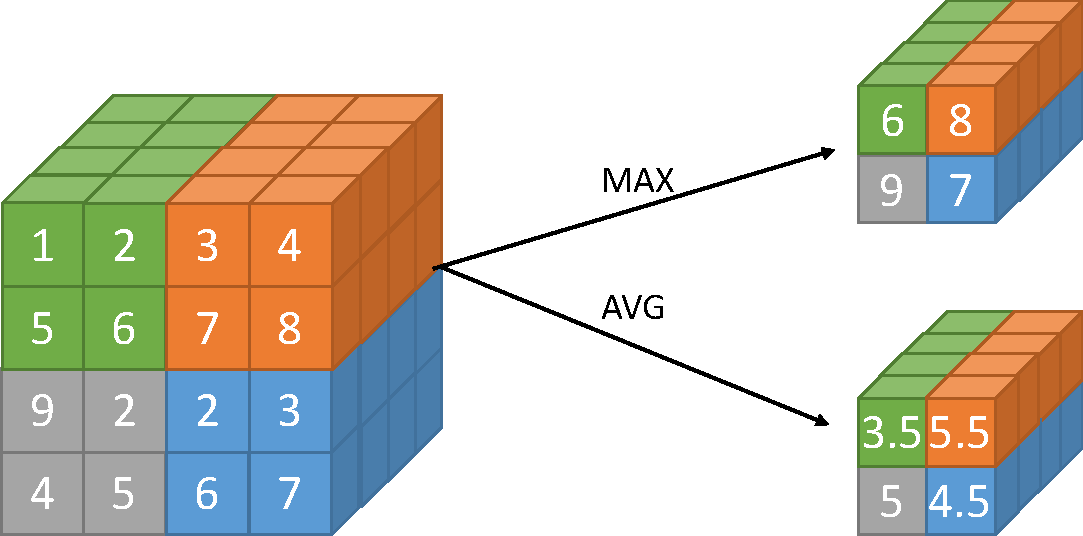
\includegraphics[width=0.6\textwidth]{pooling.pdf}
    \caption{An example of pooling layers}
    \label{fig:pool}
\end{figure}